\section{Thực nghiệm và thảo luận} % Section 3

\subsection{Kết quả phân tích}

\subsection{Biểu đồ , bảng biểu , hình ảnh minh hoạ}

\subsubsection{MobileNetV3Small}

\begin{table}[H]
\centering
\rowcolors{2}{gray!20}{white}  % tô màu từ dòng 2
\begin{tabular}{|>{\raggedright\arraybackslash}p{6cm}|c|}
\hline
\rowcolor{gray!40} \textbf{Tên kiến trúc} & \textbf{Độ chính xác (\%)} \\
\hline
MobileNetV3Small & 61.63 \\
MobileNetV3Small + FER2013 LLI & 60.49 \\
MobileNetV3Small + FER2013 LLI + adaptive augmentation & 58.15 \\
\hline
\end{tabular}
\caption{Kết quả huấn luyện}
\end{table}
    
\begin{figure}[H]
\centering
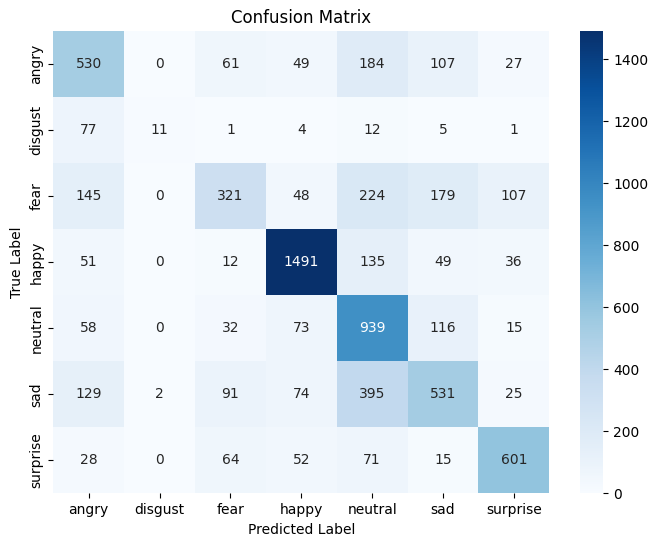
\includegraphics[width=1\textwidth]{img/confusionMatrixMobilenetV3.png}  % thay bằng tên file ảnh
\caption{Ma trận nhầm lẫn}
\end{figure}

\subsubsection{ResNet18}

\begin{table}[H]
\centering
\rowcolors{2}{gray!20}{white}  % tô xen kẽ từ dòng 2
\begin{tabular}{|>{\raggedright\arraybackslash}p{6cm}|c|}
\hline
\rowcolor{gray!40} \textbf{Tên kiến trúc} & \textbf{Độ chính xác (\%)} \\
\hline
ResNet18 & 67.23 \\
ResNet18 + FER2013 LLI & 67.04 \\
ResNet18 + FER2013 LLI + adaptive augmentation & 67.48 \\
\hline
\end{tabular}
\caption{Kết quả huấn luyện}
\end{table}

\begin{figure}[H]
\centering
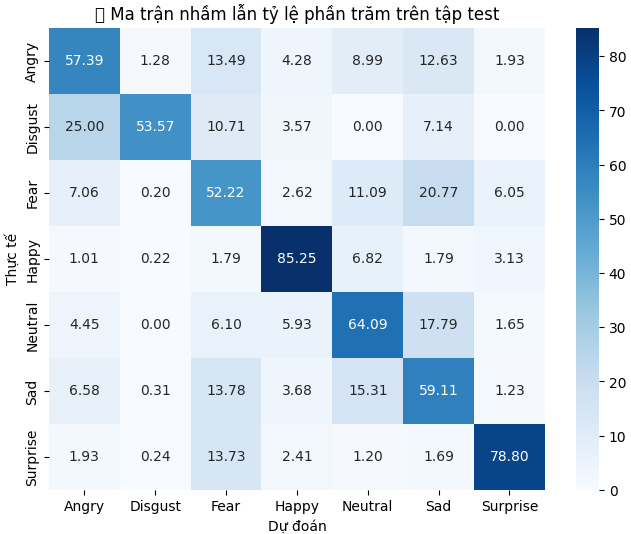
\includegraphics[width=1\textwidth]{img/confusionMatrixResnet18.png}  % thay bằng tên file ảnh
\caption{Ma trận nhầm lẫn}
\end{figure}
    
    

\subsection{Đánh giá  , giải thích kết quả nghiên  cứu}

\begin{table}[H]
\centering
\rowcolors{2}{gray!20}{white}  % tô xen kẽ từ dòng 2
\begin{tabular}{|>{\raggedright\arraybackslash}p{4cm}|l|l|l|l|}
\hline
\rowcolor{gray!40} \textbf{Tên kiến trúc} & \textbf{Accuracy (\%)} & \textbf{F1-score (\%)} & \textbf{Time infer (ms)} & \textbf{Size (MB)} \\
\hline
MobileNetV3Small & -- & -- & -- & -- \\
ResNet18 & 67.23 & 67 & 3.44 & 42.73 \\
MobileNetV3Small + FER2013 LLI  & -- & -- & -- & -- \\
ResNet18 + FER2013 LLI  & 67.04 & 67 & 3.18 & 42.72 \\
MobileNetV3Small +  FER2013 LLI +  adaptive augmentation& -- & -- & -- & -- \\
ResNet18 +  FER2013 LLI +  adaptive augmentation& 67.48 & 67 & 2.91 & 42.72 \\
\hline
\end{tabular}
\caption{Kết quả tổng thể}
\end{table}

\subsection{Nêu ý nghĩa thực tiễn của nghiên cứu}
\begin{itemize}
    \item Cải thiện độ chính xác trong điều kiện ánh sáng yếu: Hệ thống nhận diện cảm xúc thường gặp khó khăn khi môi trường thiếu sáng (ví dụ: buổi tối, trong xe hơi, phòng họp mờ...). Nghiên cứu này giúp khắc phục vấn đề đó, tăng độ tin cậy và ổn định của mô hình trong điều kiện thực tế.
    \item Giảm chi phí phần cứng: Thay vì cần máy ảnh chất lượng cao để chụp rõ trong điều kiện ánh sáng kém, việc tăng cường ảnh bằng phần mềm cho phép sử dụng thiết bị giá rẻ, phù hợp với triển khai diện rộng.
\end{itemize}

\subsection{Những hạn chế , đề xuất nghiên cứu tiếp theo}

\subsubsection{Hạn chế}
\begin{itemize}
    \item Độ chỉnh xác tổng thể còn thấp
    \item Còn nhầm lẫn giữa Disgust và Fear , Fear và Sad
    \item Đôi khi việc áp dụng kĩ thuật tăng cường có thể làm cho thời gian suy luận ảnh lâu hơn
\end{itemize}

\subsubsection{Đề xuất nghiên cứu}
\begin{itemize}
    \item Ứng dụng các mô hình học sâu để tăng cường ảnh : Thử nghiệm các phương pháp tăng cường ảnh hiện đại như Deep Image Enhancement, GANs cho ảnh ánh sáng yếu để cải thiện chất lượng đầu vào.
    \item Thu thập và mở rộng tập dữ liệu ánh sáng yếu : Xây dựng bộ dữ liệu đa dạng hơn về độ tuổi, giới tính, điều kiện ánh sáng, biểu cảm phức tạp hơn để huấn luyện và kiểm thử mô hình.
    \item Phát triển mô hình nhẹ, tối ưu thời gian suy luận : Áp dụng kỹ thuật như quantization, pruning, hoặc thiết kế lại kiến trúc nhẹ (MobileNet, EfficientNet) để giảm độ trễ khi triển khai thực tế.
\end{itemize}

